
\section{一级标题}

你可以使用如\reffig{fig:acc-no-EG-400-200}来插入图片或多幅子图。


\begin{figure}[htbp]
	\begin{minipage}[t]{0.5\linewidth}
		\centering
		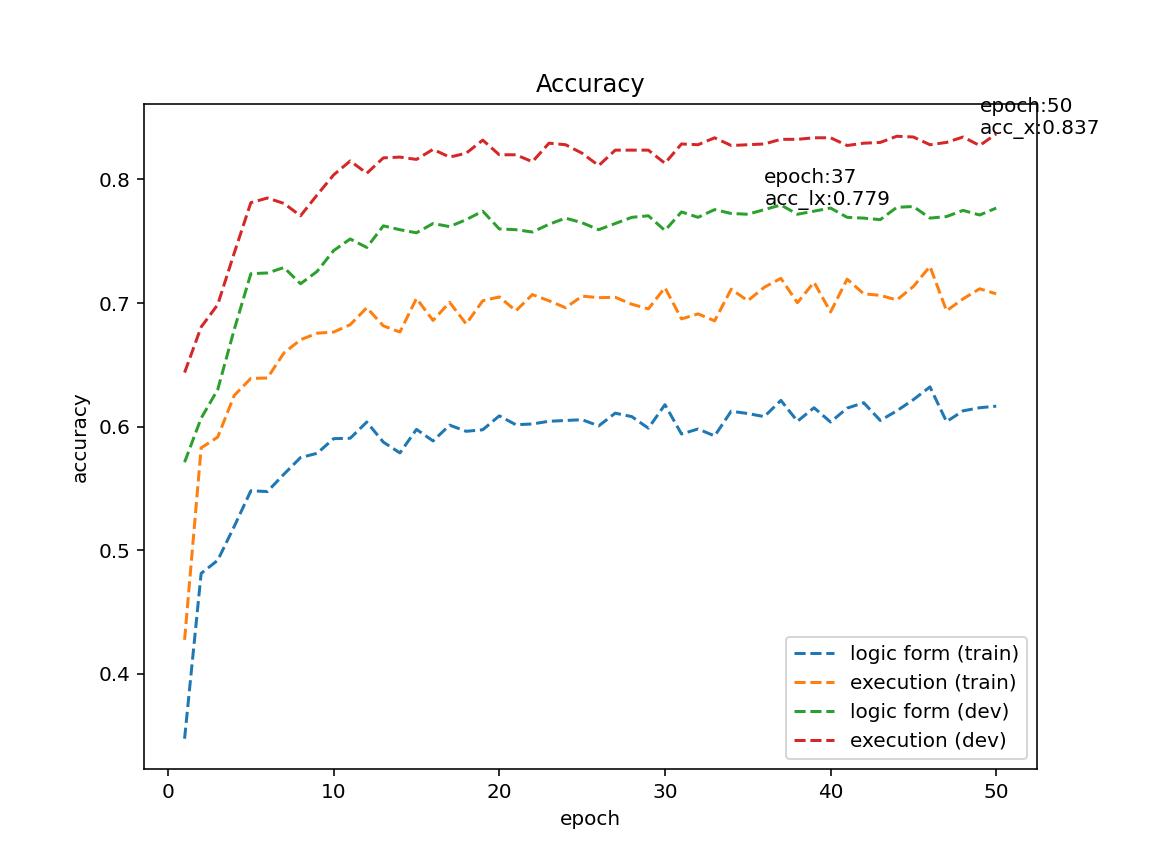
\includegraphics[width=0.99\linewidth]{.asserts/acc_NL2SQL_no_EG_400_200_e50.png}
		\text{NL2SQL-RULE}
	\end{minipage}
	\begin{minipage}[t]{0.5\linewidth}
		\centering
		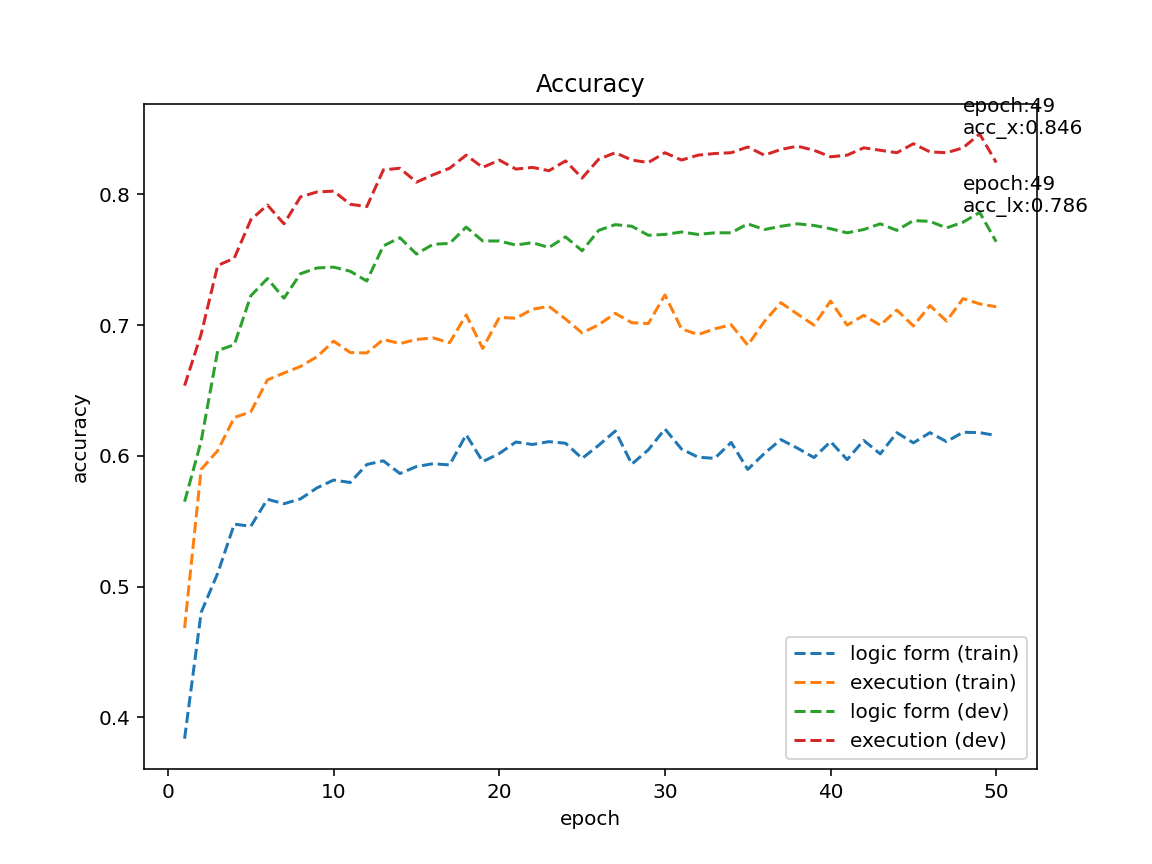
\includegraphics[width=0.99\linewidth]{.asserts/acc_ASCTEP_no_EG_400_200_e50.png}
		\text{ASCTEP(My Model)}
	\end{minipage}
	\caption{NL2SQL-RULE和ASCTEP训练过程中的准确率比较}
	\label{fig:acc-no-EG-400-200}
\end{figure}


引用文献\cite{zhongSeq2SQL2017}。如\refeq{eq:bert-wemb},这是插入公式的示例。

\begin{equation}\label{eq:bert-wemb}
	\begin{aligned}
		NLQ&=N_1, N_2, \dots, N_n \\
		hds&=hd_1, hd_2, \dots, hd_m \\
		wemb&=[CLS], N_1, N_2, \dots, N_n, [SEP], hd_1, [SEP], hd_2, \dots, [SEP], hd_m, [SEP]
	\end{aligned}
\end{equation}

如\reftab{tab:WikiSQL},这是插入表格的示例。

\begin{table}[htbp]
	\centering
	\caption{WikiSQL数据表示例}
	\label{tab:WikiSQL}
	\resizebox{\textwidth}{!}{
	\begin{tabular}{cccccc}
		\toprule
		Player & No. & Nationality & Position & Years in Toronto & \emphasize{School/Club Team}\\
		\midrule
		Antonio Lang & 21 & United States & Guard-Forward & 1999-2000 & Duke \\
		Voshon Lenard & 2 & United States & Guard & 2002-03 & Minnesota \\ 
		Martin Lewis & 32, 44 & United States & \keyword{Guard-Forward} & 1996-97 & \emphasize{Butler CC (KS)} \\
		Brad Lohaus & 33 & United States & Forward-Center & 1996 & Iowa \\
		Art Long & 42 & United States & Forward-Center & 2002-03 & Cincinnati \\
		John Long & 25 & United States & Guard & 1996-97 & Detroit \\
		Kyle Lowry & 3 & United States & Guard & 2012-Present & Villanova \\
		\bottomrule
	\end{tabular}
	}
\end{table}

如\refcode{code:code-example},这是插入代码的示例。

\begin{lstlisting}[language=python, caption={ASCTEP的AGG感知向量构造过程}, label={code:code-example}]
	question_toks = [...] # tokenized NLQ
	sql = [] # reference SQL in training
	agg_toks = [...] # tokens related to one special AGG
	
	vector = [0 for i in range(0, len(question_toks))]
	for tok in question_toks:
		if tok is superlative_adj:
			vector[indexof(tok)] = 6
		if tok in agg_toks and tok not in table_headers:
			vector[indexof(tok)] = 5
	\end{lstlisting}

\subsection{二级标题}

这是一段废话